\section{Storage Control}
\label{ch4:sec:storage-control}

In this section, the control of the energy storage system is explained.
More specifically, all parameters that are used in the Additive-Increase Multiplicative-Decrease (AIMD) algorithm are explained first.
Secondly, the structure of the BESS based AIMD algorithm is presented, where its decision mechanism is explained in full.
In the end, the voltage referencing that is used to extend AIMD to AIMD+ is detailed.

\begin{algorithm}
\KwData{$p_\text{bat}(t)$, $\text{SOC}(t)$, $v_\text{bat}(t)$, $V_\text{thr}$, $V_\text{max}$, $V_\text{min}$, $\text{SOC}_\text{max}$, $\text{SOC}_\text{min}$, $\alpha$, $\beta$}
\KwResult{$p(t + \Delta t)$}
\For{$t\leftarrow 1$ \KwTo $T$}{
	 \tcp{Define the rate for the recent voltage reading}\label{cmt}
	 $r(t) = \left(v_\text{bat}(t) - V_\text{thr}\right)$\;
	 \eIf{$v_\text{bat}(t) \geq V_\text{thr}$}{
	 	\tcp{If voltage levels are above a threshold and...}\label{cmt}
	 	\eIf{$\text{SOC}(t) \leq \text{SOC}_\text{max}$}{
	 		\tcp{...SOC is not at max.: increase charging power}\label{cmt}
	 		$p(t + \Delta t) = p_\text{bat}(t) + \alpha P_\text{max}r(t)$
	 	}{
	 		\tcp{...SOC is at max.: shut off}\label{cmt}
	 		$p(t + \Delta t) = 0$\;
	 	}
	 	\tcp{If the battery has been discharging...}\label{cmt}
	 	\If{$p_\text{bat}(t) <0$}{
		 	\tcp{...reduce discharging power by $\beta$}\label{cmt}
		 	$p(t + \Delta t) = \beta p_\text{bat}(t)$\;
	 	}
	 }{
	 	\tcp{If voltage levels are below a threshold and...}\label{cmt}
	 	\eIf{$\text{SOC}(t) \geq \text{SOC}_\text{min}$}{
	 		\tcp{...SOC is not at min.: increase discharging power}\label{cmt}
	 		$p(t + \Delta t) = p_\text{bat}(t) - \alpha P_\text{max}r(t)$
	 	}{
	 		\tcp{...SOC is at min.: shut off}\label{cmt}
	 		$p(t + \Delta t) = 0$\;
	 	}
	 	\tcp{If the battery has been charging...}\label{cmt}
	 	\If{$p_\text{bat}(t) >0$}{
		 	\tcp{...reduce charging power by $\beta$}\label{cmt}
		 	$p(t + \Delta t) = \beta p_\text{bat}(t)$\;
	 	}
	 }
	 \tcp{Restrict power to BESS limits}\label{cmt}
	 $p_\text{bat}(t + \Delta t) = \textbf{signum}(p_\text{bat}(t)) \textbf{min}(|p_\text{bat}(t)|, P_\text{max})$\;
}
\caption{Compute battery power}
\label{ch4:alg:aimd}
\end{algorithm}


\subsection{Algorithm Parameters}

\nomenclature[L]{$v_\text{bat}(t)$}{The current BESS voltage at time $t$, where $v_\text{bat}(t) \in \mathbb{R}$}
\nomenclature[L]{$\alpha$}{Control parameter that regulates the additive increase, where $\alpha \in [0, 1]$}
\nomenclature[L]{$\beta$}{Control parameter that regulates the multiplicative decrease, where $\beta \in [0, 1]$}

The proposed distributed battery storage control is shown in Algorithm~\ref{ch4:alg:aimd}.
This algorithm takes the current voltage reading, $v_\text{bat}(t)$, current BESS power, $p_\text{bat}(t)$, and the current state of charge, $\text{SOC}(t)$, as variable inputs.
Using a set of reference parameters that include the nominal voltage threshold, $V_\text{thr}$, the minimum voltage level $V_\text{min}$, the maximum voltage level, $V_\text{max}$, the minimum allowable state of charge, $\text{SOC}_\text{min}$, the maximum allowable state of charge, $\text{SOC}_\text{max}$, and the two control parameters, $\alpha$ and $\beta$, this Algorithm~\ref{ch4:alg:aimd} computes the next BESS power $p_\text{bat}(t + \Delta t)$.
The last two parameters, i.e. $\alpha$ (where $\alpha \in [0, 1]$) and $\beta$ (where $\beta \in [0, 1]$), respectively control the size of the power's additive increase step and the size of the multiplicative decrease.
In traditional Internet base applications of AIMD algorithms, $\alpha$ is set to a value that slowly increases the number of sent messages (e.g. $0.1$) and $\beta$ is set to a larger value (e.g. $0.5$) to quickly decrease throughput if congestion is noticed.
The constants $V_\text{max}$, $V_\text{min}$ and $V_\text{thr}$ are the maximum and minimum historic voltage values and the set-point threshold that is used to regulate the BESS operation.
In the case when the total demand is too high, the local voltages will fall below $V_\text{thr}$, and the batteries reduce their charging power and eventually start discharging.
This behaviour raises overall voltage levels since the total demand on the feeder is reduces.
For the simulations in this chapter, $V_\text{max}$ is set to the nominal voltage of the substation transformer, i.e., 240 V, and $V_\text{thr}$ is set to a value below $V_\text{max}$, which was found by solving a balanced power flow analysis of the underlying network.
For each BESS, $V_\text{min}$ is then chosen as the value below $V_\text{thr}$ so that $V_\text{thr}$ lies equidistant to $V_\text{max}$ and $V_\text{min}$.
The variable $v_\text{bat}(t)$ is the battery's local bus voltage and is used to trigger control actions.
This value is obtained by solving the power flow of the underlying network and adjusts the battery power, $p_\text{bat}(t)$, in as defined in by the algorithm.
To stay within operational limits, $P_\text{max}$ is set as the maximum charging/discharging power of the battery.
The charging and discharging power of the batteries is increased in proportion to the available headroom on the network (which is inferred from the local voltage measurement $v_\text{bat}(t)$) to avoid any sudden overloading of the substation transformer.

\subsection{AIMD Algorithm Structure}

The algorithm itself, as shown in Algorithm~\ref{ch4:alg:aimd}, contains two decision levels.
The first level (lines 4-17) determines whether the network is underloaded by comparing the local bus voltage, $v_\text{bat}(t)$, to the battery's set-point threshold, $V_\text{thr}$.
If the network is under low load, i.e. when $v_\text{bat}(t) \geq V_\text{thr}$, then the BESS is triggered to decrease its power injection until it begins charging.
In this case, the battery's SOC is compared to its operation limit to check whether the battery can charge, i.e., $\text{SOC}$ \textless $\text{SOC}_\text{max}$.
If there is enough charging capacity left, then the battery's charging power is linearly increased using $\alpha$ (lines 6-8).
Otherwise, i.e. if the BESS is fully charged by reaching its highest charge level of $\text{SOC}_{max}$, the charging process is turned off (lines 9-11).
If the battery was previously discharging however, the related discharging power is multiplicatively reduced (lines 14-17) to begin reducing voltage levels.

The second decision level (lines 18-32) is entered when the network is overloaded.
If the network is under high load, i.e. when $v_\text{bat}(t) < V_\text{thr}$, then the BESS is triggered to decrease its charging power until it begins to inject energy into the network. 
In this case, the discharging power is linearly increased if the battery has enough energy stored, i.e. $\text{SOC}$ \textgreater $\text{SOC}_\text{min}$ (lines 20-22).
Otherwise, i.e. if the BESS has discharged to its low charge level of $\text{SOC}_{min}$, the discharging process is turned off (lines 23-25).
However, if the battery was previously charging, then its charging power is multiplicatively reduced (line 28-31) to begin increasing voltage levels.

The direction of the charging/discharging power adjustment is determined by the first decision level, as well as the threshold proximity ratio $r(t)$.
As the battery's bus voltage, $v_\text{bat}(t)$, approaches the threshold voltage, $V_\text{thr}$, this ratio tends to zero and thus stops the battery operation.
Therefore, oscillatory hunting is effectively mitigated.
The last step of the algorithm (lines 33-34) assures that the battery's charge/discharge power stays within the device's ratings.

\subsection{Reference Voltage Profile}

The difference in the location and load of each customer results in the over-utilisation of the batteries that are located at the feeder end.
This is particularly true when using a fixed voltage threshold.
To individualise the voltage thresholds, a reference voltage profile is generated by performing a power flow analysis of the network model by subjecting it to its maximum power demand.
This approach is comparable to the procedure by Papaioannou et al. in \cite{Papaioannou2015} who generated profiles for the control of EV charging.
In this chapter however, bi-directional power flow of BESS is controlled.
An example of a fixed threshold and reference voltage profile is shown in Figure~\ref{ch4:fig:ref-voltage-difference}.

\begin{figure}\centering
	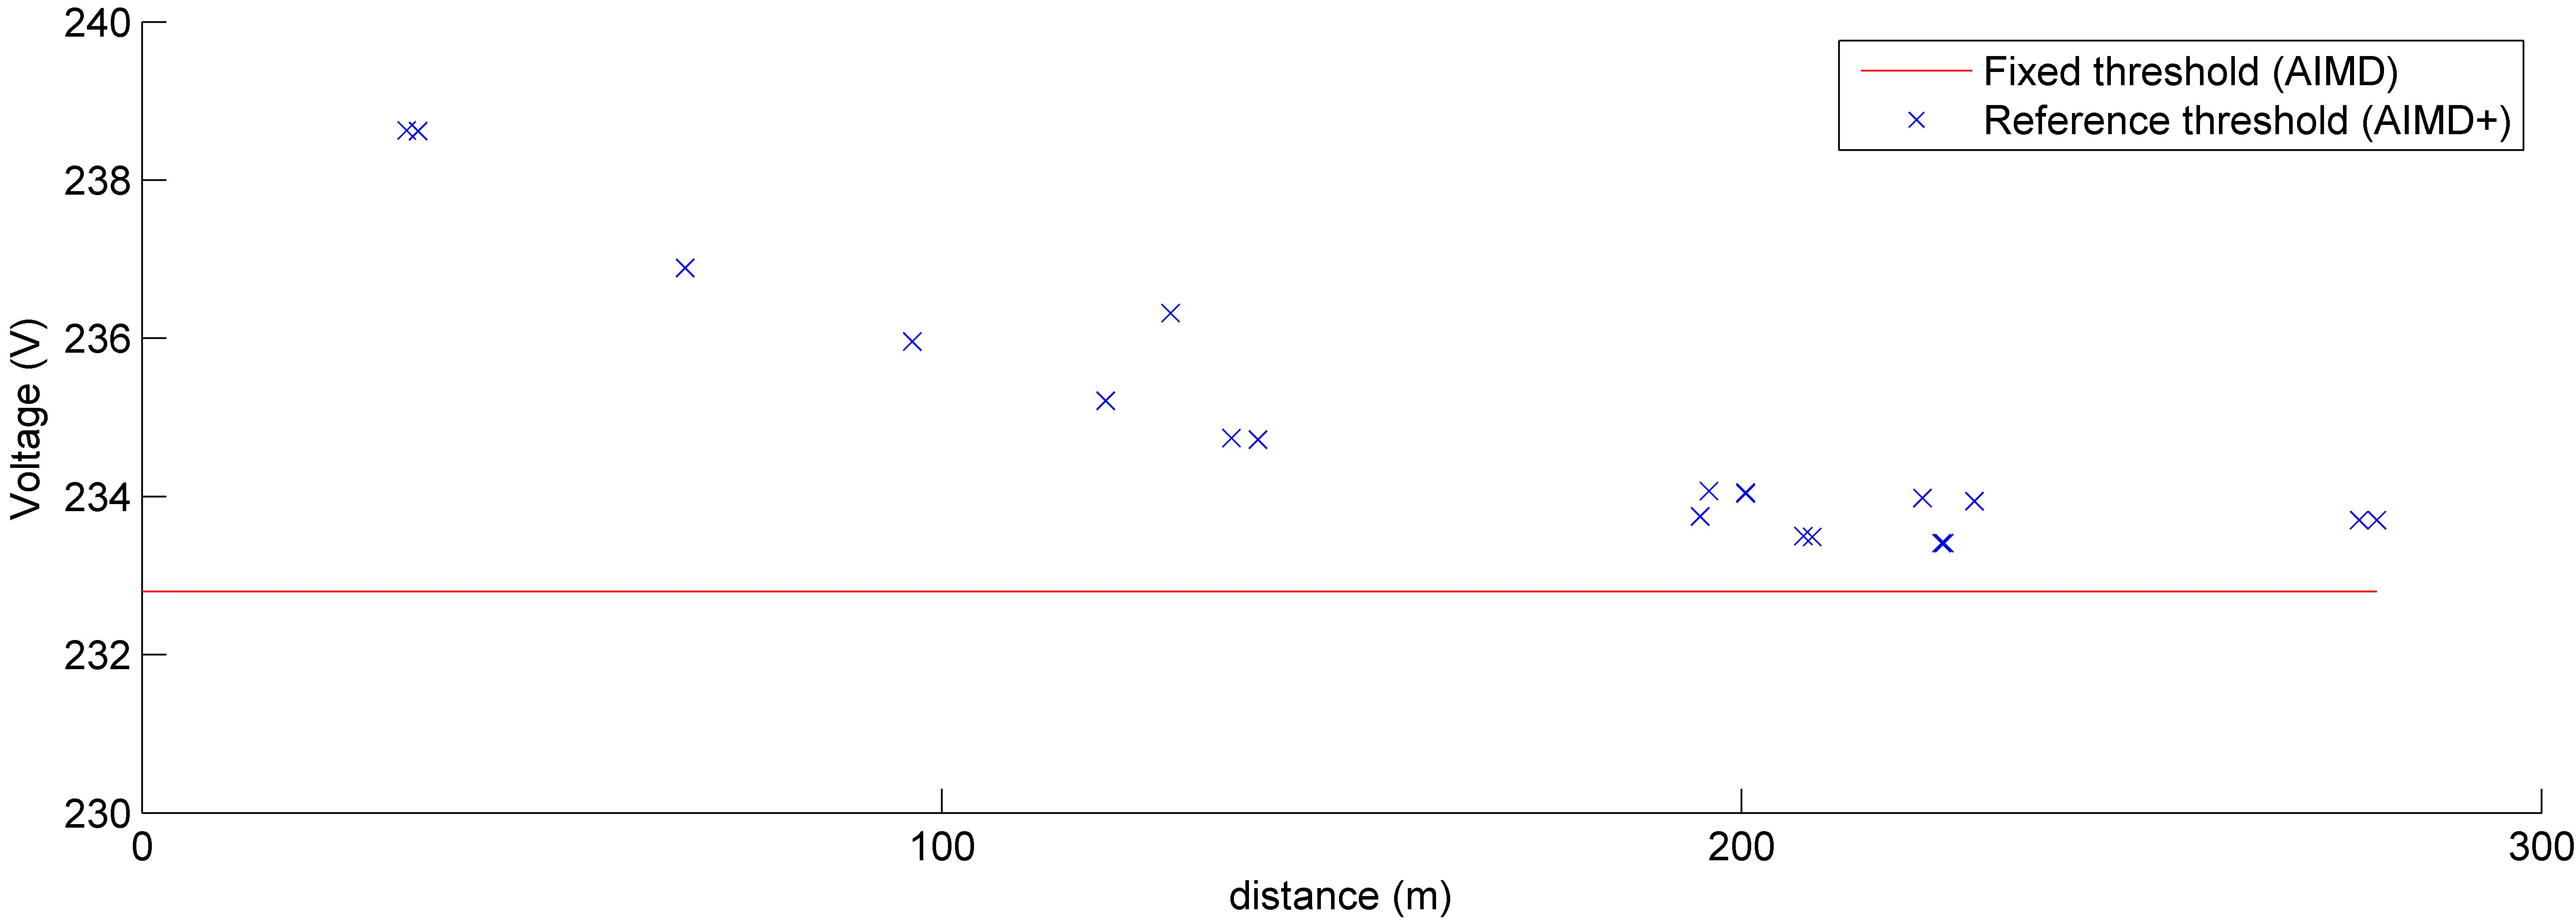
\includegraphics{_chapter4/fig/ref-voltage-difference}
	\caption{A plot showing the difference between the fixed voltage threshold (AIMD) and the reference voltage profile (AIMD+).}
	\label{ch4:fig:ref-voltage-difference}
\end{figure}

Therefore, in the AIMD+, consumers located at the head of the feeder are allocated a higher voltage threshold than those towards the end of the feeder.
However, customers with lower thresholds are allocated a voltage threshold similar to that of the fixed threshold control.
This allocation takes into account the expected voltage drop, that occurs along the length of the feeder, and hence results in a better tuned utilisation of all battery storage units, regardless of their distance to the substation.
For the work presented in this chapter, the voltage threshold is set in such a way as to limit the maximum voltage drop to 3\% at the end of the feeder.


